\section{Technologies Used}
\subsection{iOS}
iOS is a mobile operating system, created and developed by Apple \cite{iOS}. It is the operating system that currently runs on many of the company's devices, such as iPhone, iPad, or iPod Touch. It is considered to be the second most popular mobile operating system, after Android \cite{iOS}.

\subsection{Swift}
Swift is a programming language created by Apple, which was launch as an alternative for Objective-C, in order to create iOS apps \cite{swift}. The goal of the creators of Swift is to create a programming language that could be used on a variety of systems, such as mobile, desktop or even cloud services (servers) \cite{swift}. Soon after the launch, the programming language has been made open-source, which has opened the way for it to be used in more than just iOS-running devices. Swift is believed to be:
\begin{itemize}
    \item Safe
    \item Fast: it was made as a replacement for C-based languages, which have always been very fast.
    \item Expressive: "Swift benefits from decades of advancement in computer science to offer syntax that is a joy to use, with modern features developers expect" \cite{swift}.
\end{itemize}

Because this is the most popular way to create iOS applications, Swift has been chosen in order to make the user and admin applications.

\subsection{Vapor}
Vapor is a web framework that provides a way to create server side applications using Swift. It is a secure framework, which offers encryption for all network requests as default, and a very fast framework. Benchmarks have been showing that it is nearly 100 times faster that other web frameworks, such as Ruby and PHP \cite{vapor}. Due to its rapid rise and popularity and its very helping community, this framework has been chosen as an experiment in order to determine how feasible it is to create web applications using Swift.

\subsection{Python}
Python is a interpreted programming languages, meant to be used for general-purpose programming. Python is very easy to learn and use, regardless of the programmer's experience \cite{python}. This programming languages will be used for the AR Data Provider, mainly due to the fact that there are a multitude of libraries that achieve most of the tasks one would like. The vast number of community-contributed modules allow for "endless possibilities" \cite{python}. In our project, the Selenium library will be used in order to effortlessly automate actions in a web browser, when using King's timetable service.

\subsection{Flask}
Flask is a lightweight microframework for Python \cite{flask}. This allows to write server applications using Python. The framework makes possible creating the server that will provide data for the AR features in the user application. Because the design is very decoupled, this framework makes the connection between the AR Data Provider and any system that requires its data.

\subsection{Linux}
Linux is a family of free and open-source operating systems. It is a very popular system that runs on a variety of platforms, from phones to desktop computers, and to servers and mainframe computers \cite{linux}. The Raspberry Pi runs a light distribution of Linux, called Raspbian. This operating systems offers basic functionalities for the Raspberry Pi devices, and it is made to be very optimised for low-performance processors.

\subsection{Java}
Java is a general-purpose programming language that was inspired by C++ and is more focused on the object-oriented side of programming. It is one of the most popular programming languages in use. Java apps can run on any Java virtual machine, regardless of the operating system, or architecture. Because it is very popular and very widely used, this programming language has been chosen for the Raspberry Pi application.

\subsection{ARKit}
ARKit is a framework that allows programmers to bring AR experiences in their iOS applications \cite{arkit}. It was launched together with iOS 11 and makes using AR on iOS much more easier than before. The framework provides a lot of functionalities that the developers can easily use, such as scene understanding and lightning estimations, which detects the vertical and horizontal panes which are around, and makes use of the camera to detect the amount of light available and later apply it to the virtual objects \cite{arkit}. This framework has been chosen because of its ease of use on iOS and its high level of performance optimisation.

\subsection{Heroku}
Heroku is a cloud platform that allows web applications to be deployed. It supports a vast number of programming languages and frameworks, mainly because its active community. Heroku brings a very easy and simple solution for deployment and has been chosen as a solution in our project mainly because of this reason.

\subsection{PostgreSQL}
PostgreSQL is a relational database system, based on SQL \cite{postgresql}. It currently runs on most of the major operating systems, and is supported by the majority of programming languages \cite{postgresql}. Because the servers have been deployed on Heroku, and because Heroku supports PostgreSQL as its main relational database system, this component has been chosen for our project.

\newpage
\section{Architectural Design}
The architecture has been divided into four independent layers. This approach makes the whole system easier to manage, and very simple to replace or change parts of it, if they need to be extended or improved. The System Architecture Diagram shown in figure \ref{fig:system-architecture-design}, describes the aforementioned four layers. 

The top layer, the User Interface Layer, is composed of the two applications: the admin application, used to measure and register positions in Bush House, and the user application, which will make use of the data for positioning and navigation. 
The second layer, the Scanning Layer, deals with scanning data when requested (when recording a position or when positioning is needed) and uploading it in the database. This layer is composed of a Raspberry Pi that scans, parses results and makes HTTP requests in order to upload the data, and a simple web application that will act as a bridge between the Raspberry Pi and the mobile applications, by letting the Raspberry Pi know when data is needed.

The lower two layers, the Logic Layer and the Data Management Layer, work together to receive, process and provide data for the User Interface Layer. Data is saved by the Data Management Layer which has an API that acts as an interface for the database. The Logic Layer processes available data in order to come up with the most optimal route to get from point A to point B, to determine the current position, or to provide data to be used for AR, such as timetables or the number of available PCs.

\begin{figure}[H]
    \centering
    \fbox{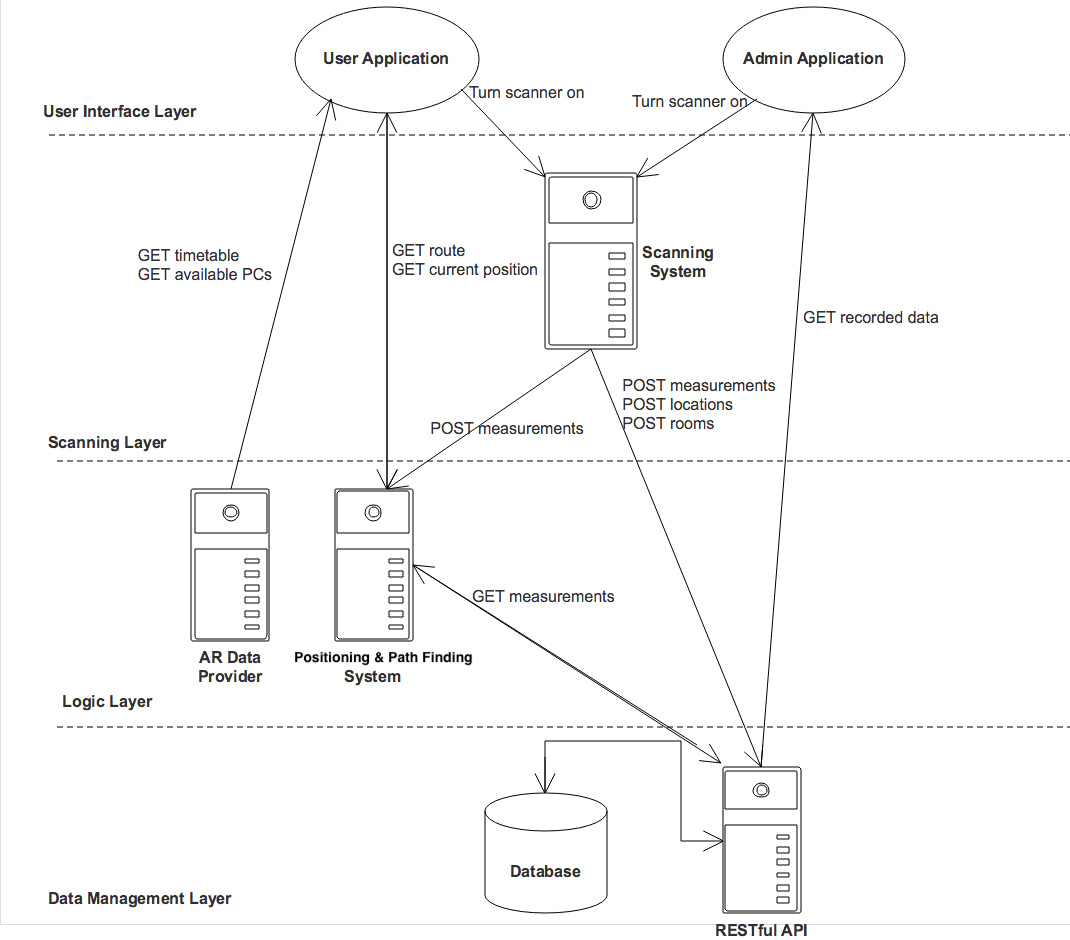
\includegraphics[width=420px, height=360px]{Design/diagram2.png}}
    \centering
    \caption{System Architecture Design. Depicts the 4 layers of the navigation system, along with the subsystems and how they interact between themselves.}
    \label{fig:system-architecture-design}
\end{figure}

\subsection{User Interface Layer Overview}
The user interface layer will act as a front-end to the system, and will deal with all user specific tasks. Due to the nature of tasks that need to be accomplished, this layer has been divided into two separate applications. One single application could have been developed, but for the sake of simplicity and avoiding a user-based system, they have been separated. The admin application is meant to be used as a measurement tool in order to record locations for the rooms in Bush House, whereas the user application will be used by any user who would want navigation assistance for Bush House, without having write permissions for the database, as the admin application has.

\subsubsection{Admin Application}
The admin application has been designed using the Model-View-Controller (MVC\nomenclature{MVC}{Model-View-Controller}) architectural pattern. MVC is the go-to architectural pattern that is used when developing iOS application, therefore our app is following it as well. The model handles all the data processing and fetching, whereas the controller converts the data from the model and shows it in the view. The application uses components already defined in UIKit, which is the framework for user interface elements in iOS. The whole architecture of the application is described in figure \ref{fig:admin-mvc}. The code of the each component of each element of MVC will be detailed in chapter 5, the Implementation chapter, and it will be fully available in the Appendix.

\begin{figure}[H]
    \centering
    \fbox{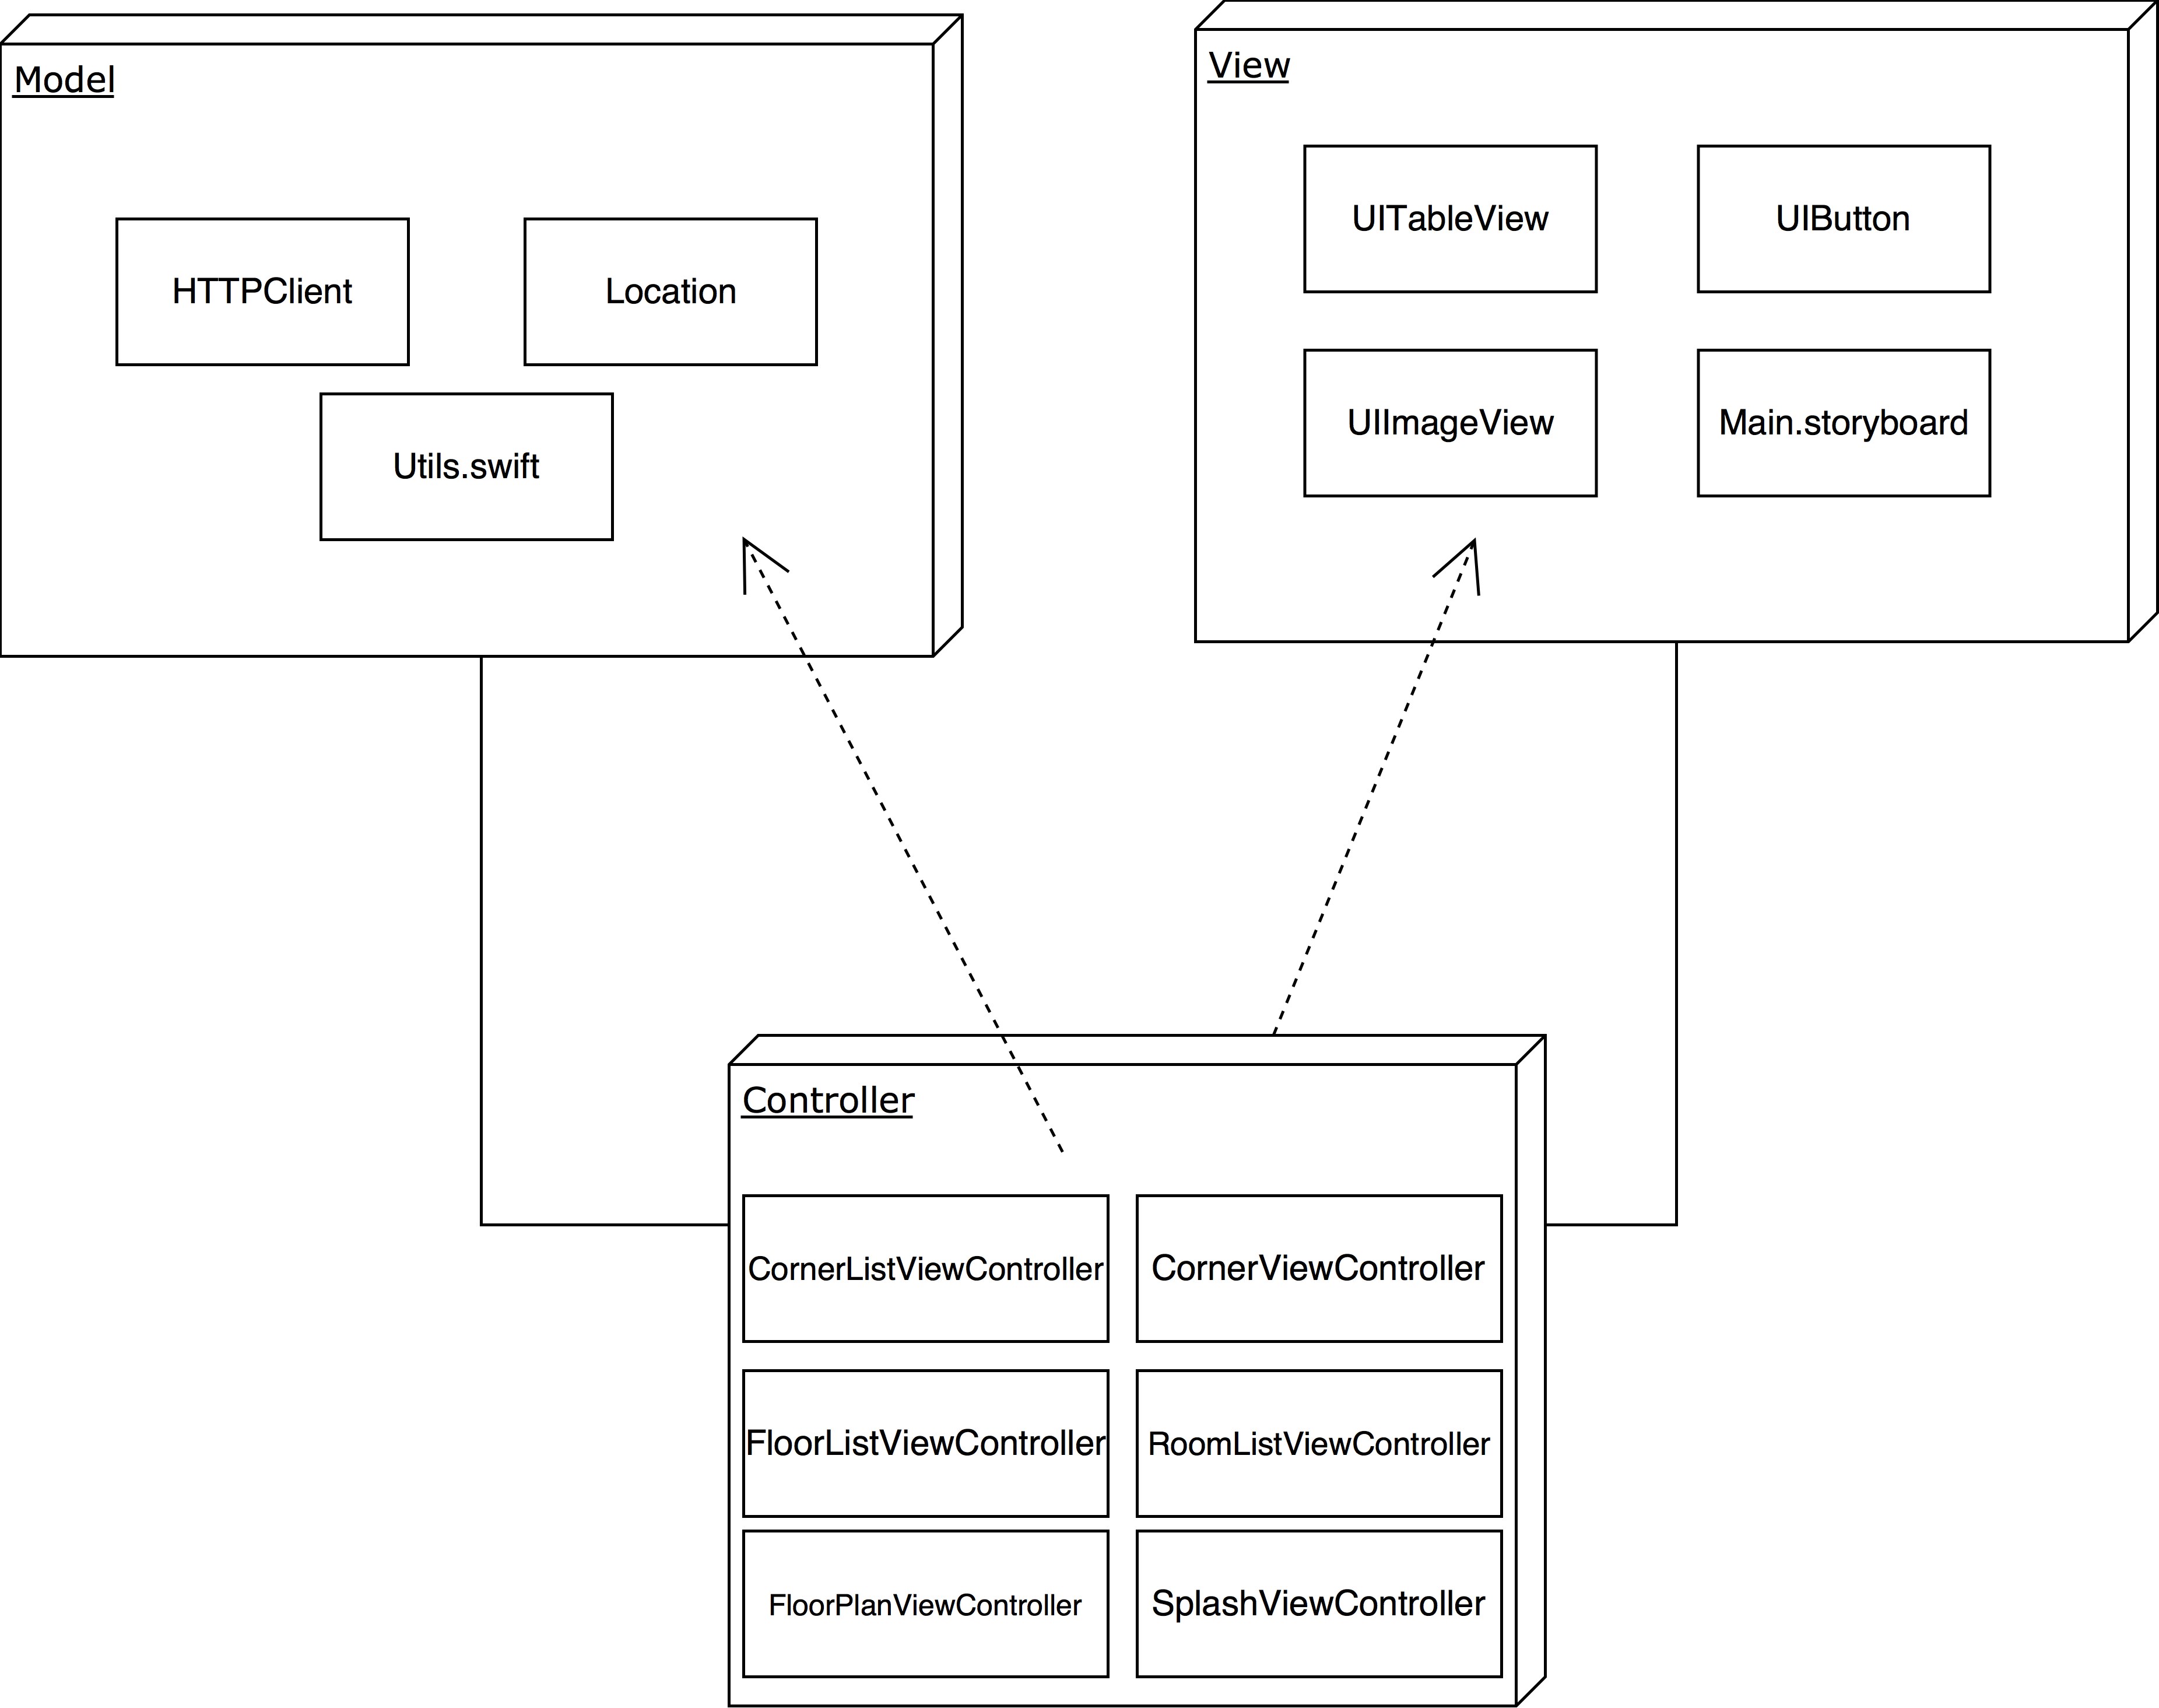
\includegraphics[width=420px, height=332px]{Design/Admin-MVC.png}}
    \centering
    \caption{Admin Application MVC Design. The design is split into model, view and controller. The rectangles inside each component represent the classes that are part of it.}
\label{fig:admin-mvc}
\end{figure}

Upon the first launch of the application, the admin user will be required to calibrate the application. This process involves registering the corners of the mobile device's screen. The values registered will come into play when using triliteration (see section \ref{sec:triliteration}) to calculate the values of the positions measured in latitude and longitude, in the following way:

\begin{itemize}
    \item The values on the screen of the corners of the floor plan will be measured by the admin, by tapping on the screen.
    \item Then, the values from the 2D plan (the screen) are assigned to the positions in latitude and longitude of the corners of the building that are already entered in the application.
    \item Now, any position from the 2D plan can be translated into latitude and longitude using triliteration, following these steps:
    \begin{itemize}
        \item Three corners are chosen and the distances between them in the 2D plan are calculated. The distance in meters is calculated after using the haversine formula (see section \ref{sec:haversine}).
        \item The distance in the 2D plan from the three corners to the measured location is calculated.
        \item The distance in meters from the corners to the chosen point is found. This is done by translating the known distances calculated in the first step.
        \item Using triliteration, the values in latitude and longitude of the chosen point are found.
    \end{itemize}
\end{itemize}

After the position is calculated both in 2D values, and latitude and longitude, the application must upload them into the database, using the API.

\subsubsection{User Application}
The user application is designed following an MVC pattern as well. The components of MVC achieve similar goals as the admin application. 

\begin{figure}[H]
    \centering
    \fbox{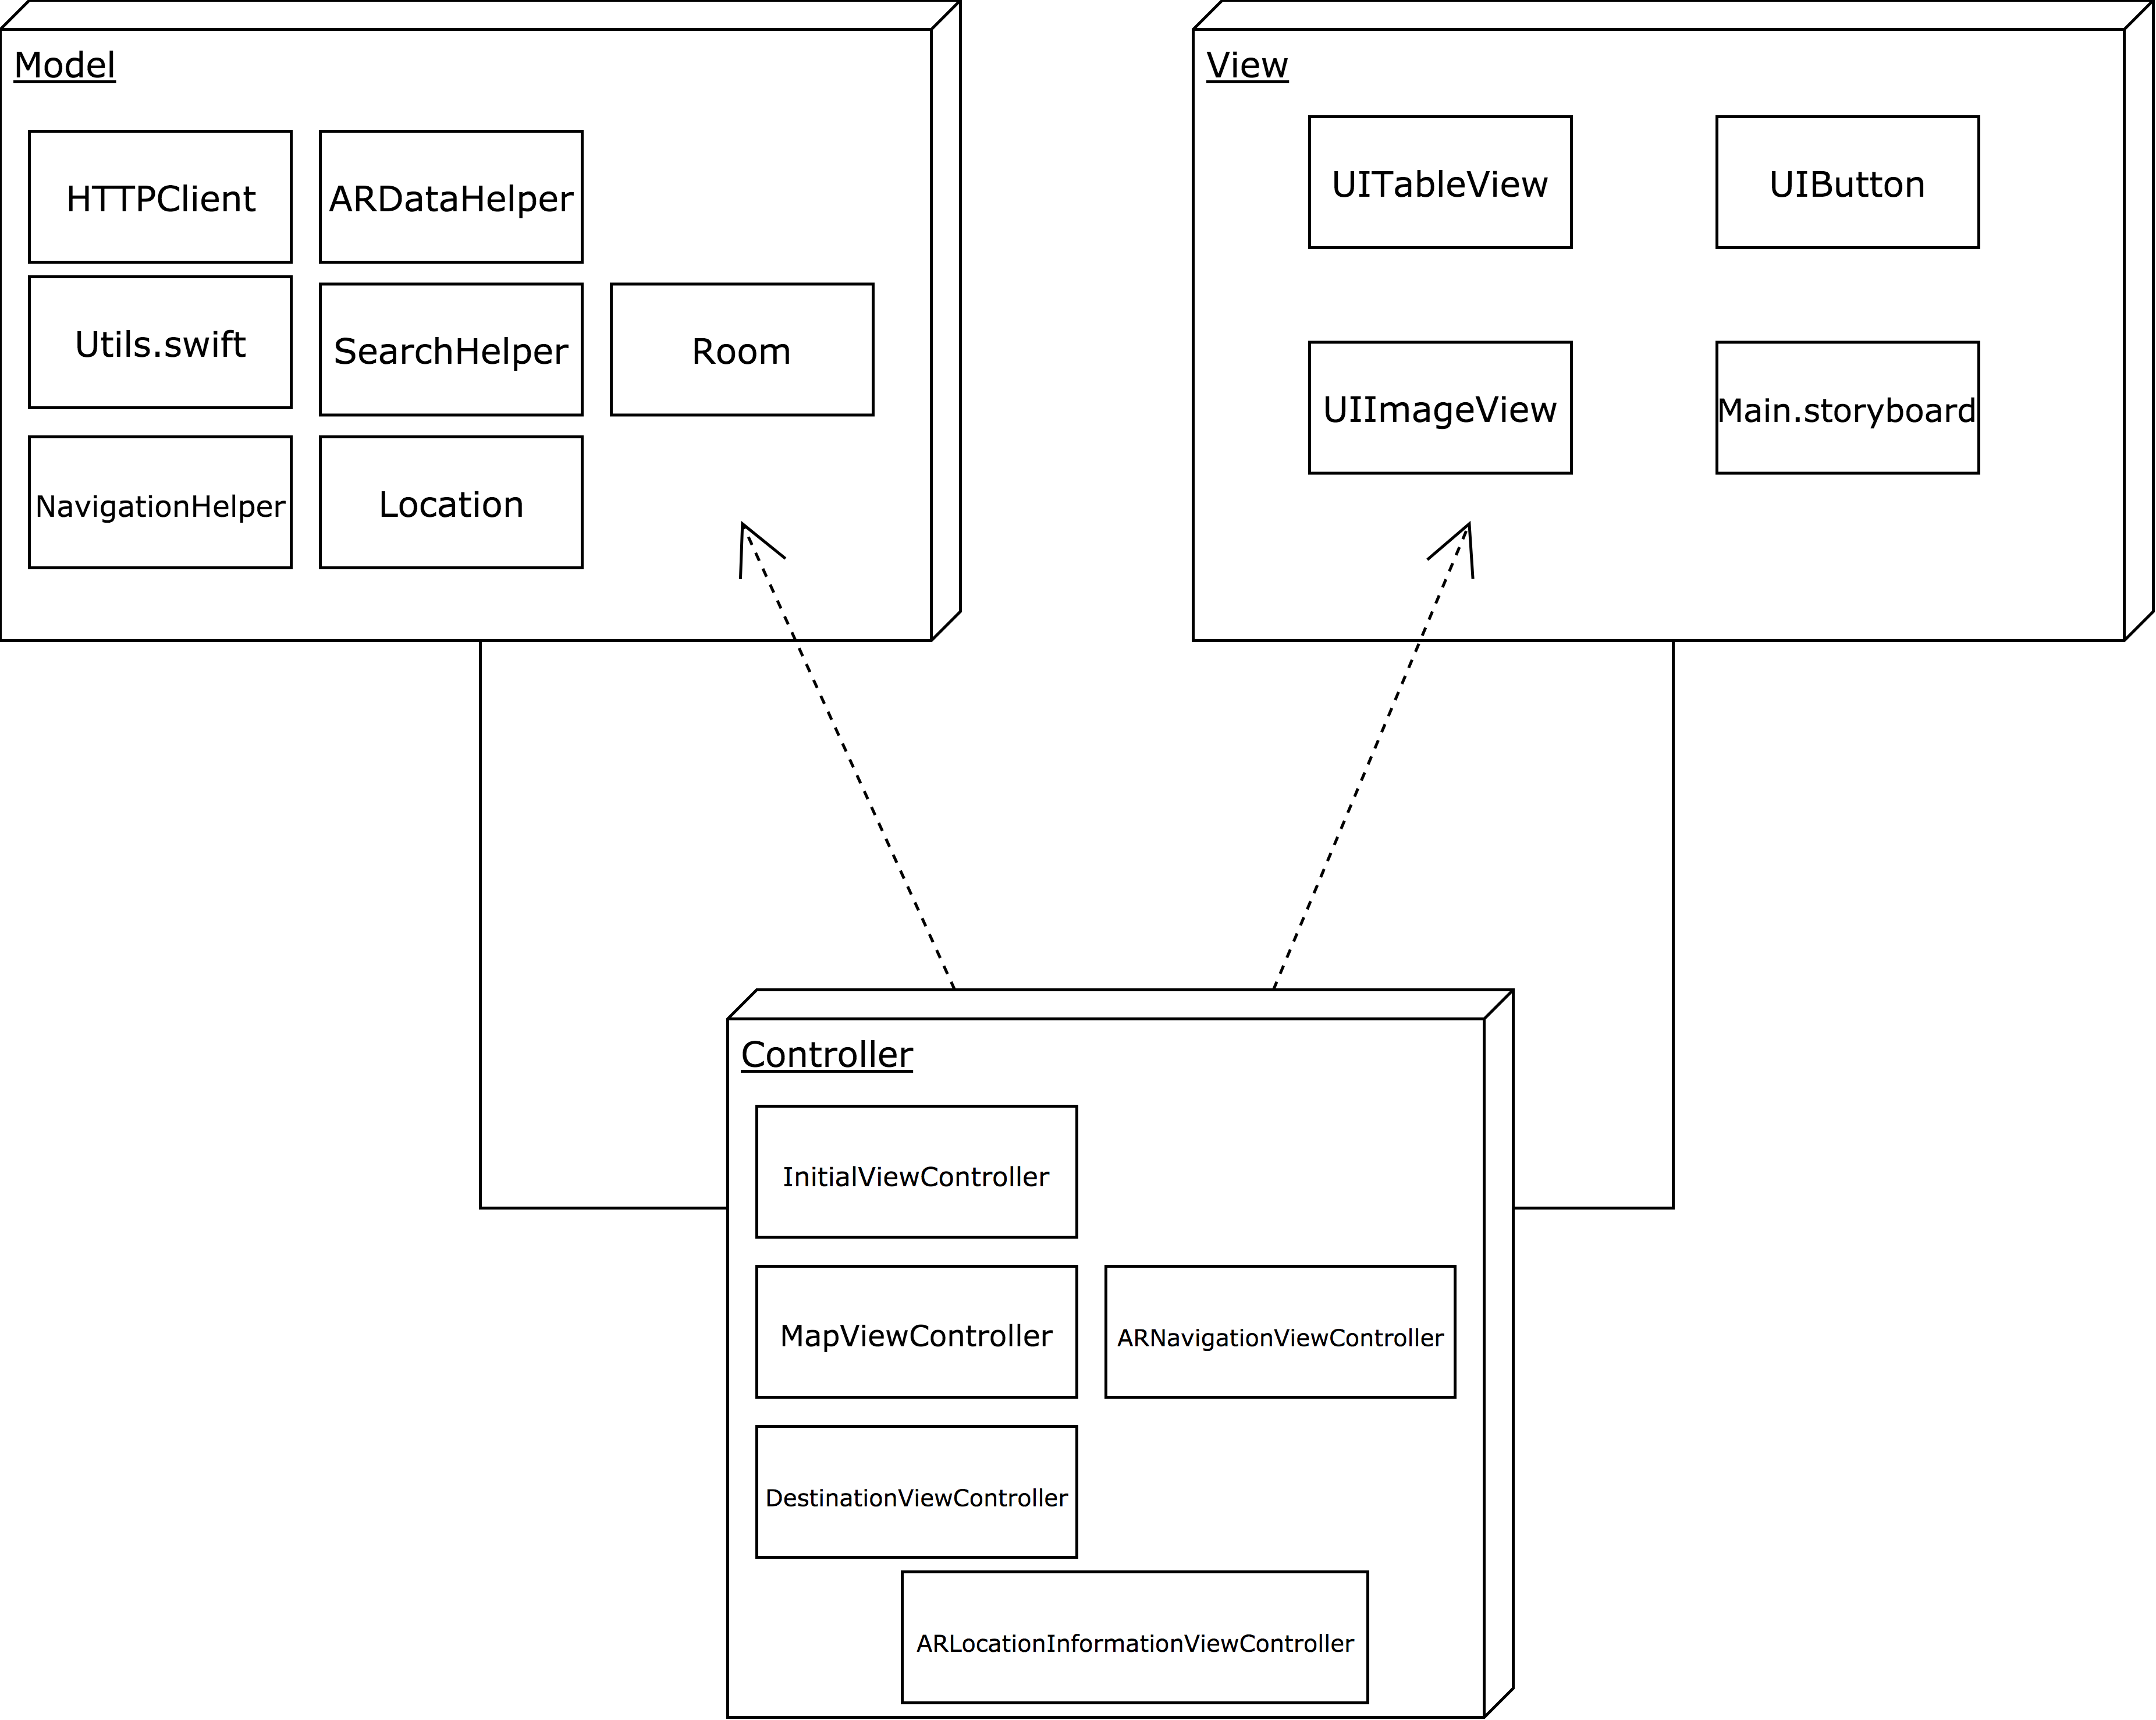
\includegraphics[width=420px, height=335px]{Design/User-MVC.png}}
    \centering
    \caption{User Application MVC Design. The design is split into model, view and controller. The rectangles inside each component represent the classes that are part of it.}
    \label{fig:user-mvc}
\end{figure}

The user application will greet the user by calculating their current position by showing a dot on the floor plan that belongs to the floor they are currently on. From there, the user can view a list of possible destinations and by selecting one, a path will be shown on the screen on how to get there. Another action that the user can make is using the AR features. The AR features are:
\begin{itemize}
    \item Images of timetables will render and placed in the rooms that are around.
    \item The number of computers will also be shown and placed in the rooms that are around.
\end{itemize}
One important matter to mention is how the AR objects will be placed. Based on the user's current location, the closest locations to each room that are around are calculated. By using those and the ARKit+CoreLocation library, the AR objects will be placed on the corresponding Location objects, using their latitude and longitude values.

\subsection{Scanning Layer}
The scanner layer will handle measuring for Wi-Fi signal strengths and uploading them in the database when needed. This layer is comprised of two applications: the scanner which will run on a Raspberry Pi, and a small web application that will handle the scan requests between the mobile applications and the Raspberry Pi.

\subsubsection{Raspberry Pi Scanner Application}
The first application is a Java application managed by a Linux script that runs every 2 seconds and implements the following functions:
\begin{itemize}
    \item Scan and store Wi-Fi networks found around using Linux system commands.
    \item Check if the data needs to be uploaded.
    \item If yes, upload data onto the back-end storage, and then set the need to scan flag to off.
    \item If not, don't do anything.
    \item Run the above mentioned set of steps every 2-3 seconds.
\end{itemize}

\subsubsection{Scanner Switch Application}

The second part of the scanning layer is a small web application that acts as a switch. The Scanner Switch Application is going to be developed using Vapor, a Swift framework which follows an MVC pattern as well (see figure \ref{fig:scan-switch-mvc}). Although this design pattern has been used traditionally for applications that have a graphical user interface, it has become popular for web applications as well. In this case, the application runs on a server, without a graphical user interface, so the JSON takes the role of the View component in this case.

\begin{figure}[H]
    \centering
    \fbox{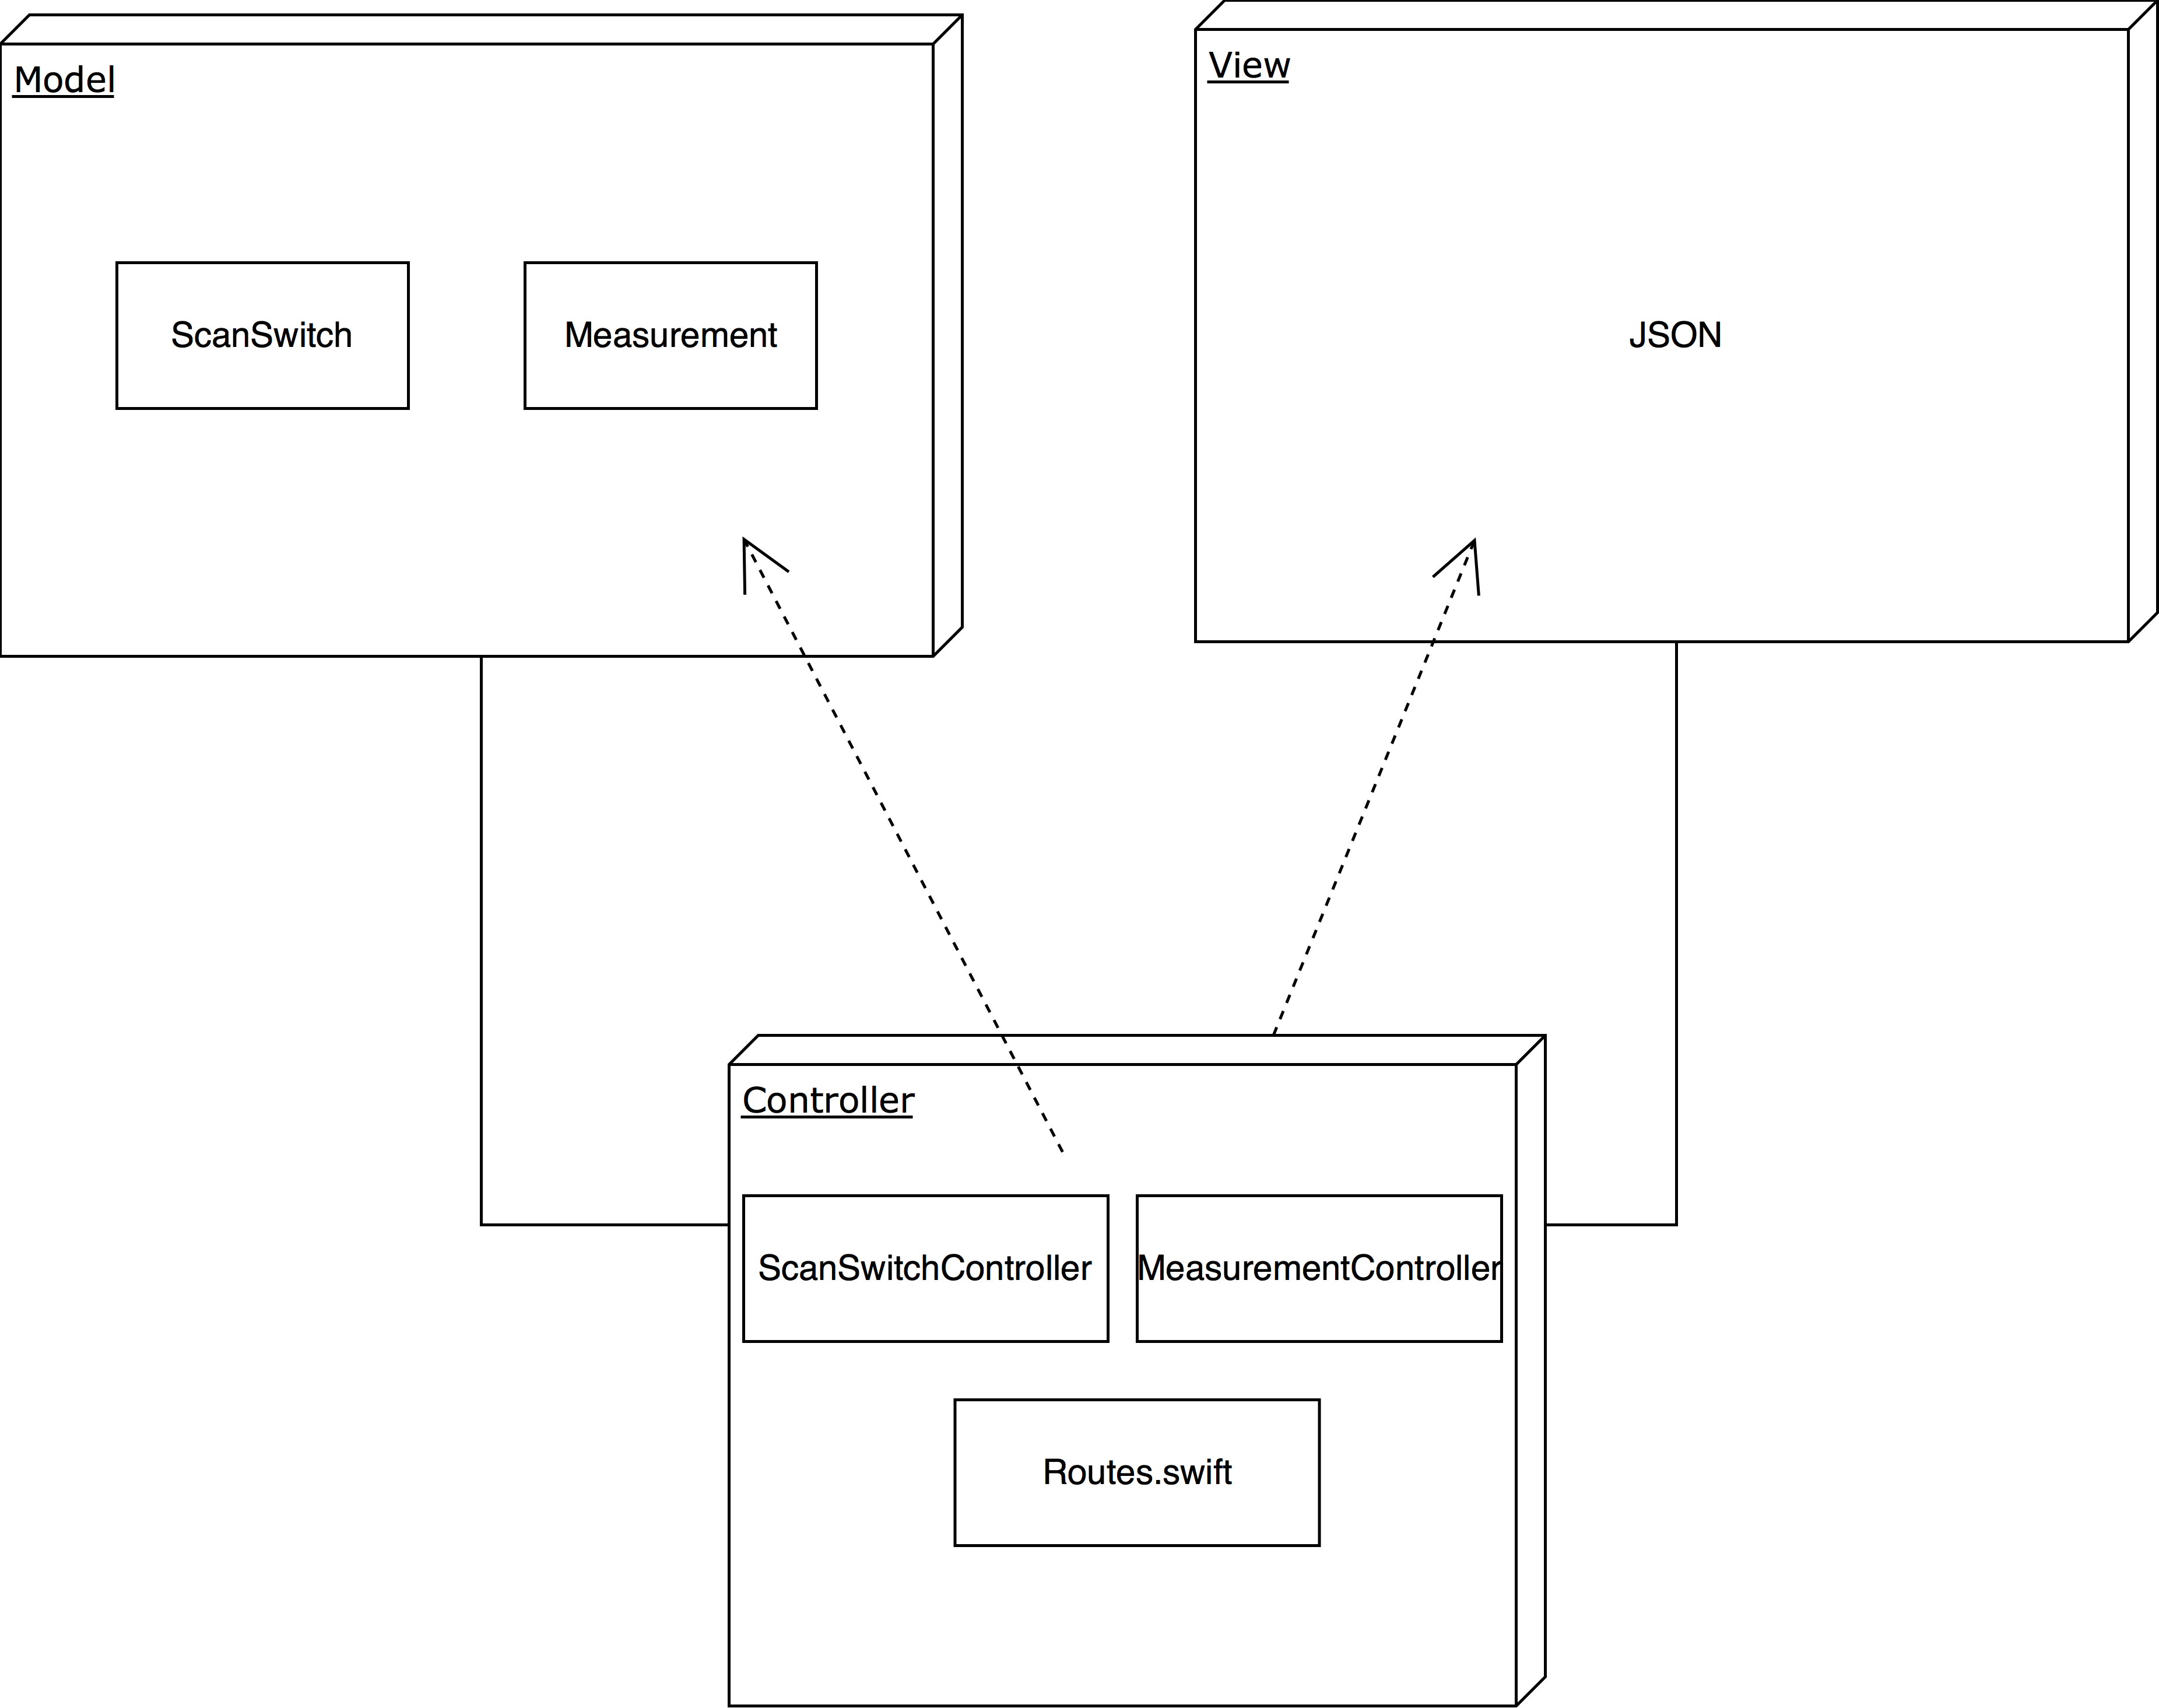
\includegraphics[width=420px, height=332px]{Design/Scan-Switch-MVC.png}}
    \centering
    \caption{Scan Switch MVC Design. The design is split into model, view and controller. The rectangles inside each component represent the classes that are part of it.}
\label{fig:scan-switch-mvc}
\end{figure}

The goal of this application is to let the scanning application on the Raspberry Pi know if data is needed or not. The data is stored in an in-memory database which will contain the following fields:
\begin{itemize}
    \item scanSwitch: Can be true or false, depending if data is needed or not.
    \item locationID: This will be used when uploading data in the database in order to link Measurement objects to a Location object.
    \item roomID: This value will be used to link the Location object for which the Measurement objects are scanned to a room.
    \item storeData: Can be true or false, if the data needs to be stored or not. For example, when measuring locations the data needs to be scanned, but when the scanned data is used only for navigation or positioning, the data doesn't need to be saved. If the data doesn't need to be saved, the measurements will be temporarily stored on this server, and then discarded after the positioning process has finished.
\end{itemize}

This application implements a REST API that handles HTTP requests in order to access the data. HTTP requests are made to "http://address/resource", where resource is the resource targeted. The following resources are available:
\begin{itemize}
    \item For resource "/scanSwitch/1":
    \begin{itemize}
        \item PATCH: Updates the values of the aforementioned fields.
    \end{itemize}
    
    \item For resource "/measurements":
    \begin{itemize}
        \item POST: Creates a temporarily stored measurement.
        \item DELETE: Deletes all the measurements.
    \end{itemize}
\end{itemize}

\subsection{Logic Layer}
The Logic Layer is composed of two systems: the AR data provider and the positioning \& path finding system. These two subsystems provide the core algorithms and functions that the system relie on. 

\subsubsection{Positioning \& Path Finder System}
This part of the project is the most important one, because the positioning and path finder system calculates all the data to position the user and find optimal paths. Because it will developed using Vapor, as we will see in the Implementation chapter, it follows an MVC design pattern. Similar as before, the View component is here represented by the JSON responses, as we will see shortly.

\begin{figure}[H]
    \centering
    \fbox{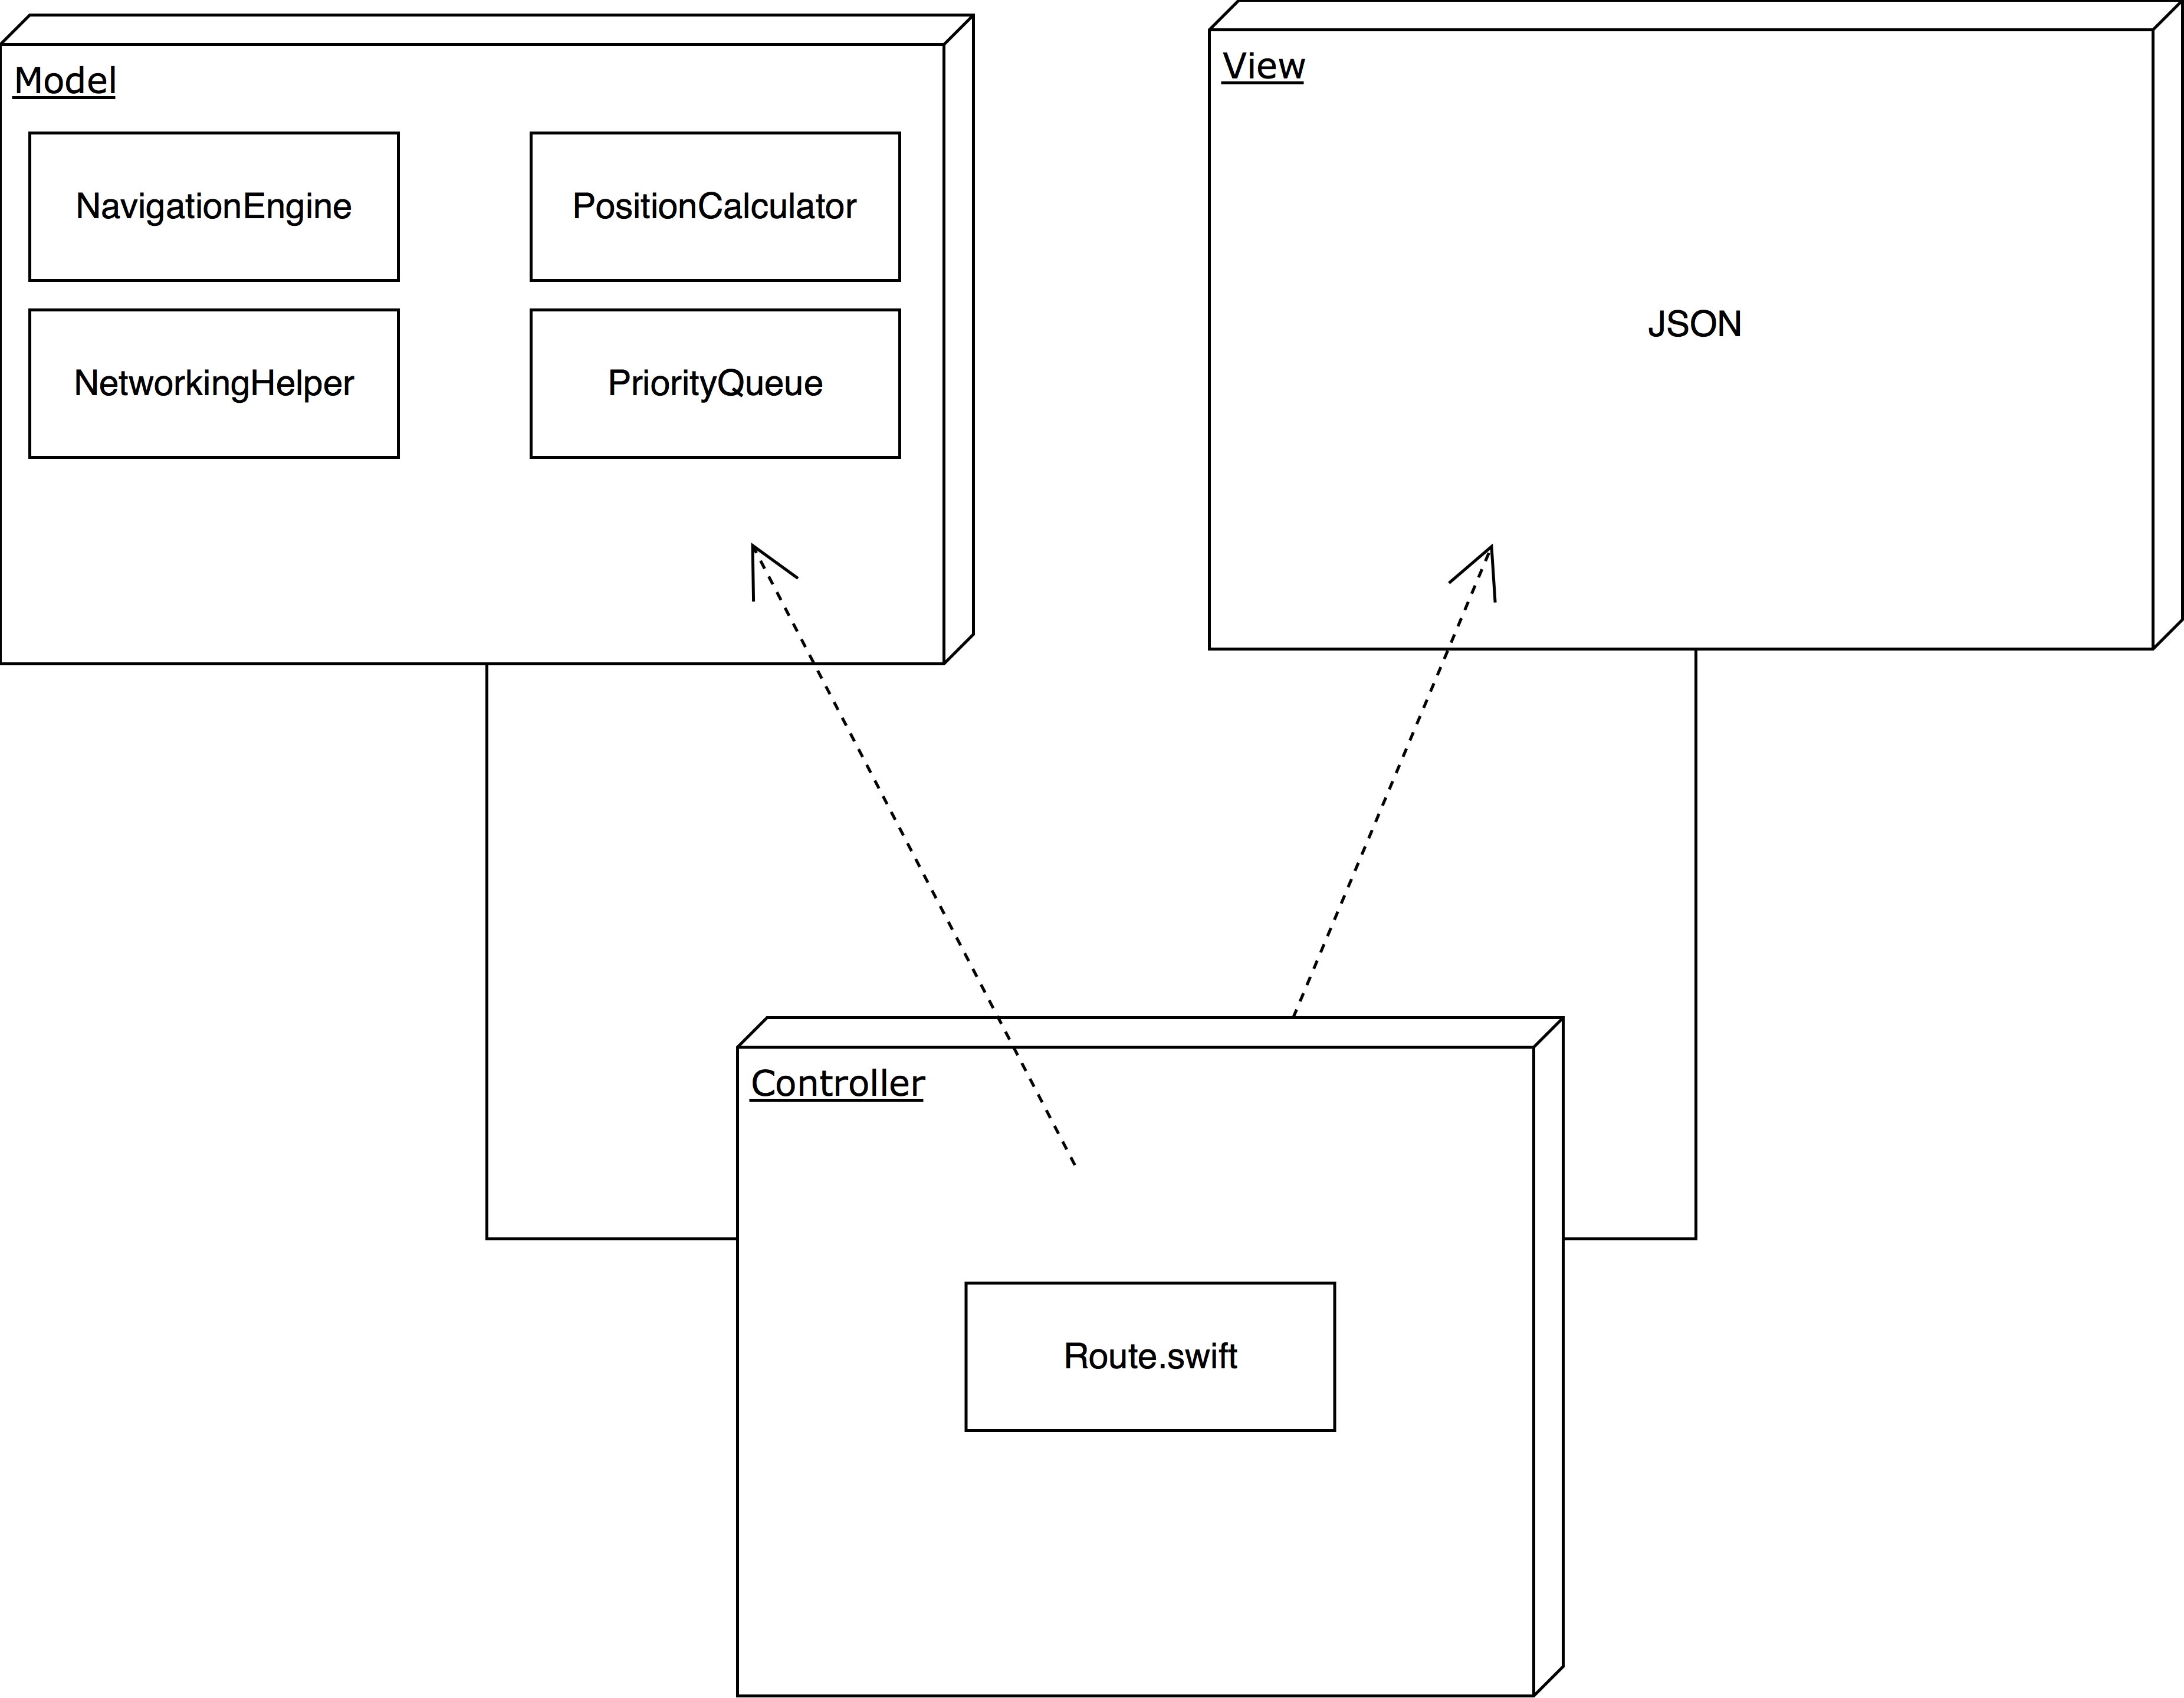
\includegraphics[width=386px, height=300px]{Design/Back-end-MVC.png}}
    \centering
    \caption{Positioning \& Path Finder System MVC Design. The design is split into model, view and controller. The rectangles inside each component represent the classes that are part of it.}
    \label{fig:pos-nav-mvc}
\end{figure}

The positioning algorithm will be based on a best match algorithm, working as follows:
\begin{itemize}
    \item For each measurement received, query the database and find all the past measurements recorded from the corresponding Wi-Fi access point.
    \item Calculate the difference in signal strengths between the current measurement and the past one.
    \item Find the location that has the minimum difference from all the differences calculated.
    \item Keep count of how many times locations have matched.
    \item At the end, find the location with the most matches.
\end{itemize}

Finding routes will be done using Dijkstra's algorithm, described in section \ref{sec:dijkstra}. A graph will be built using the data from the database, and based on that, the shortest path will be calculated. The end result will be a list of location IDs to follow along with the total distance of the path. 

This system implements an API to retrieve the calculated data, such as the current position. The API handles HTTP requests to "http://address/resource", where "resource" is the targeted resource. The resources available to access are the following:
\begin{itemize}
    \item For resource "/determinePosition":
    \begin{itemize}
        \item POST: accepts an array of current measurements and returns a JSON object of a location that has the 2D coordinates along with latitude and longitude
    \end{itemize}
    
    \item For resource "/calculateRoute":
    \begin{itemize}
        \item POST: accepts a JSON object that includes a "startLocationID" and a "finishLocationID" which represent the start and finish locations of the desired route. The return result will be a JSON object that is made of the distance of the path, along with an array of the location IDs to follow to get from start to finish.
    \end{itemize}
\end{itemize}

% Here need to say what the components will be and how the system is going to actually do stuff, but on a design wise level so no code, classes etc.

\subsubsection{AR Data Provider}
The AR Data Provider will consist of an application that will be able to parse data from the university timetable system and from PC-Free@King's which provides how many computers are in the computer labs. Unfortunately, PC-Free has data for only one room located in Bush House, so not all rooms will be supported. This limitation has been detailed in section \ref{sec:limitations}. The data will be obtained through a RESTf API, which, as before described with the previous APIs, handles HTTP requests made to certain resources:
\begin{itemize}
    \item For resource "/timetable/[roomCode]":
    \begin{itemize}
        \item GET: Returns a JPG image of the timetable for the current week, for the specified room.
    \end{itemize}
    
    \item For resource "pcfree/[roomCode]":
    \begin{itemize}
        \item GET: Returns how many computers are available in the specified room, and if there are not any, returns "No computers are available".
    \end{itemize}
\end{itemize}

\subsection{Data Management Layer}
The Data Management Layer holds and manages the data which the logic layer uses. This layer is ran using a Vapor server that manages a PostgreSQL database. Similarly to the previous logic layer, the database can be accessed through an API. Due to the fact that the implementation is done using Vapor, the design is done by using an MVC patter, shown in figure \ref{fig:back-end-storage-mvc}. As before, the View component here is represented by the JSON responses from the API that is going to be detailed below.

\begin{figure}[H]
    \centering
    \fbox{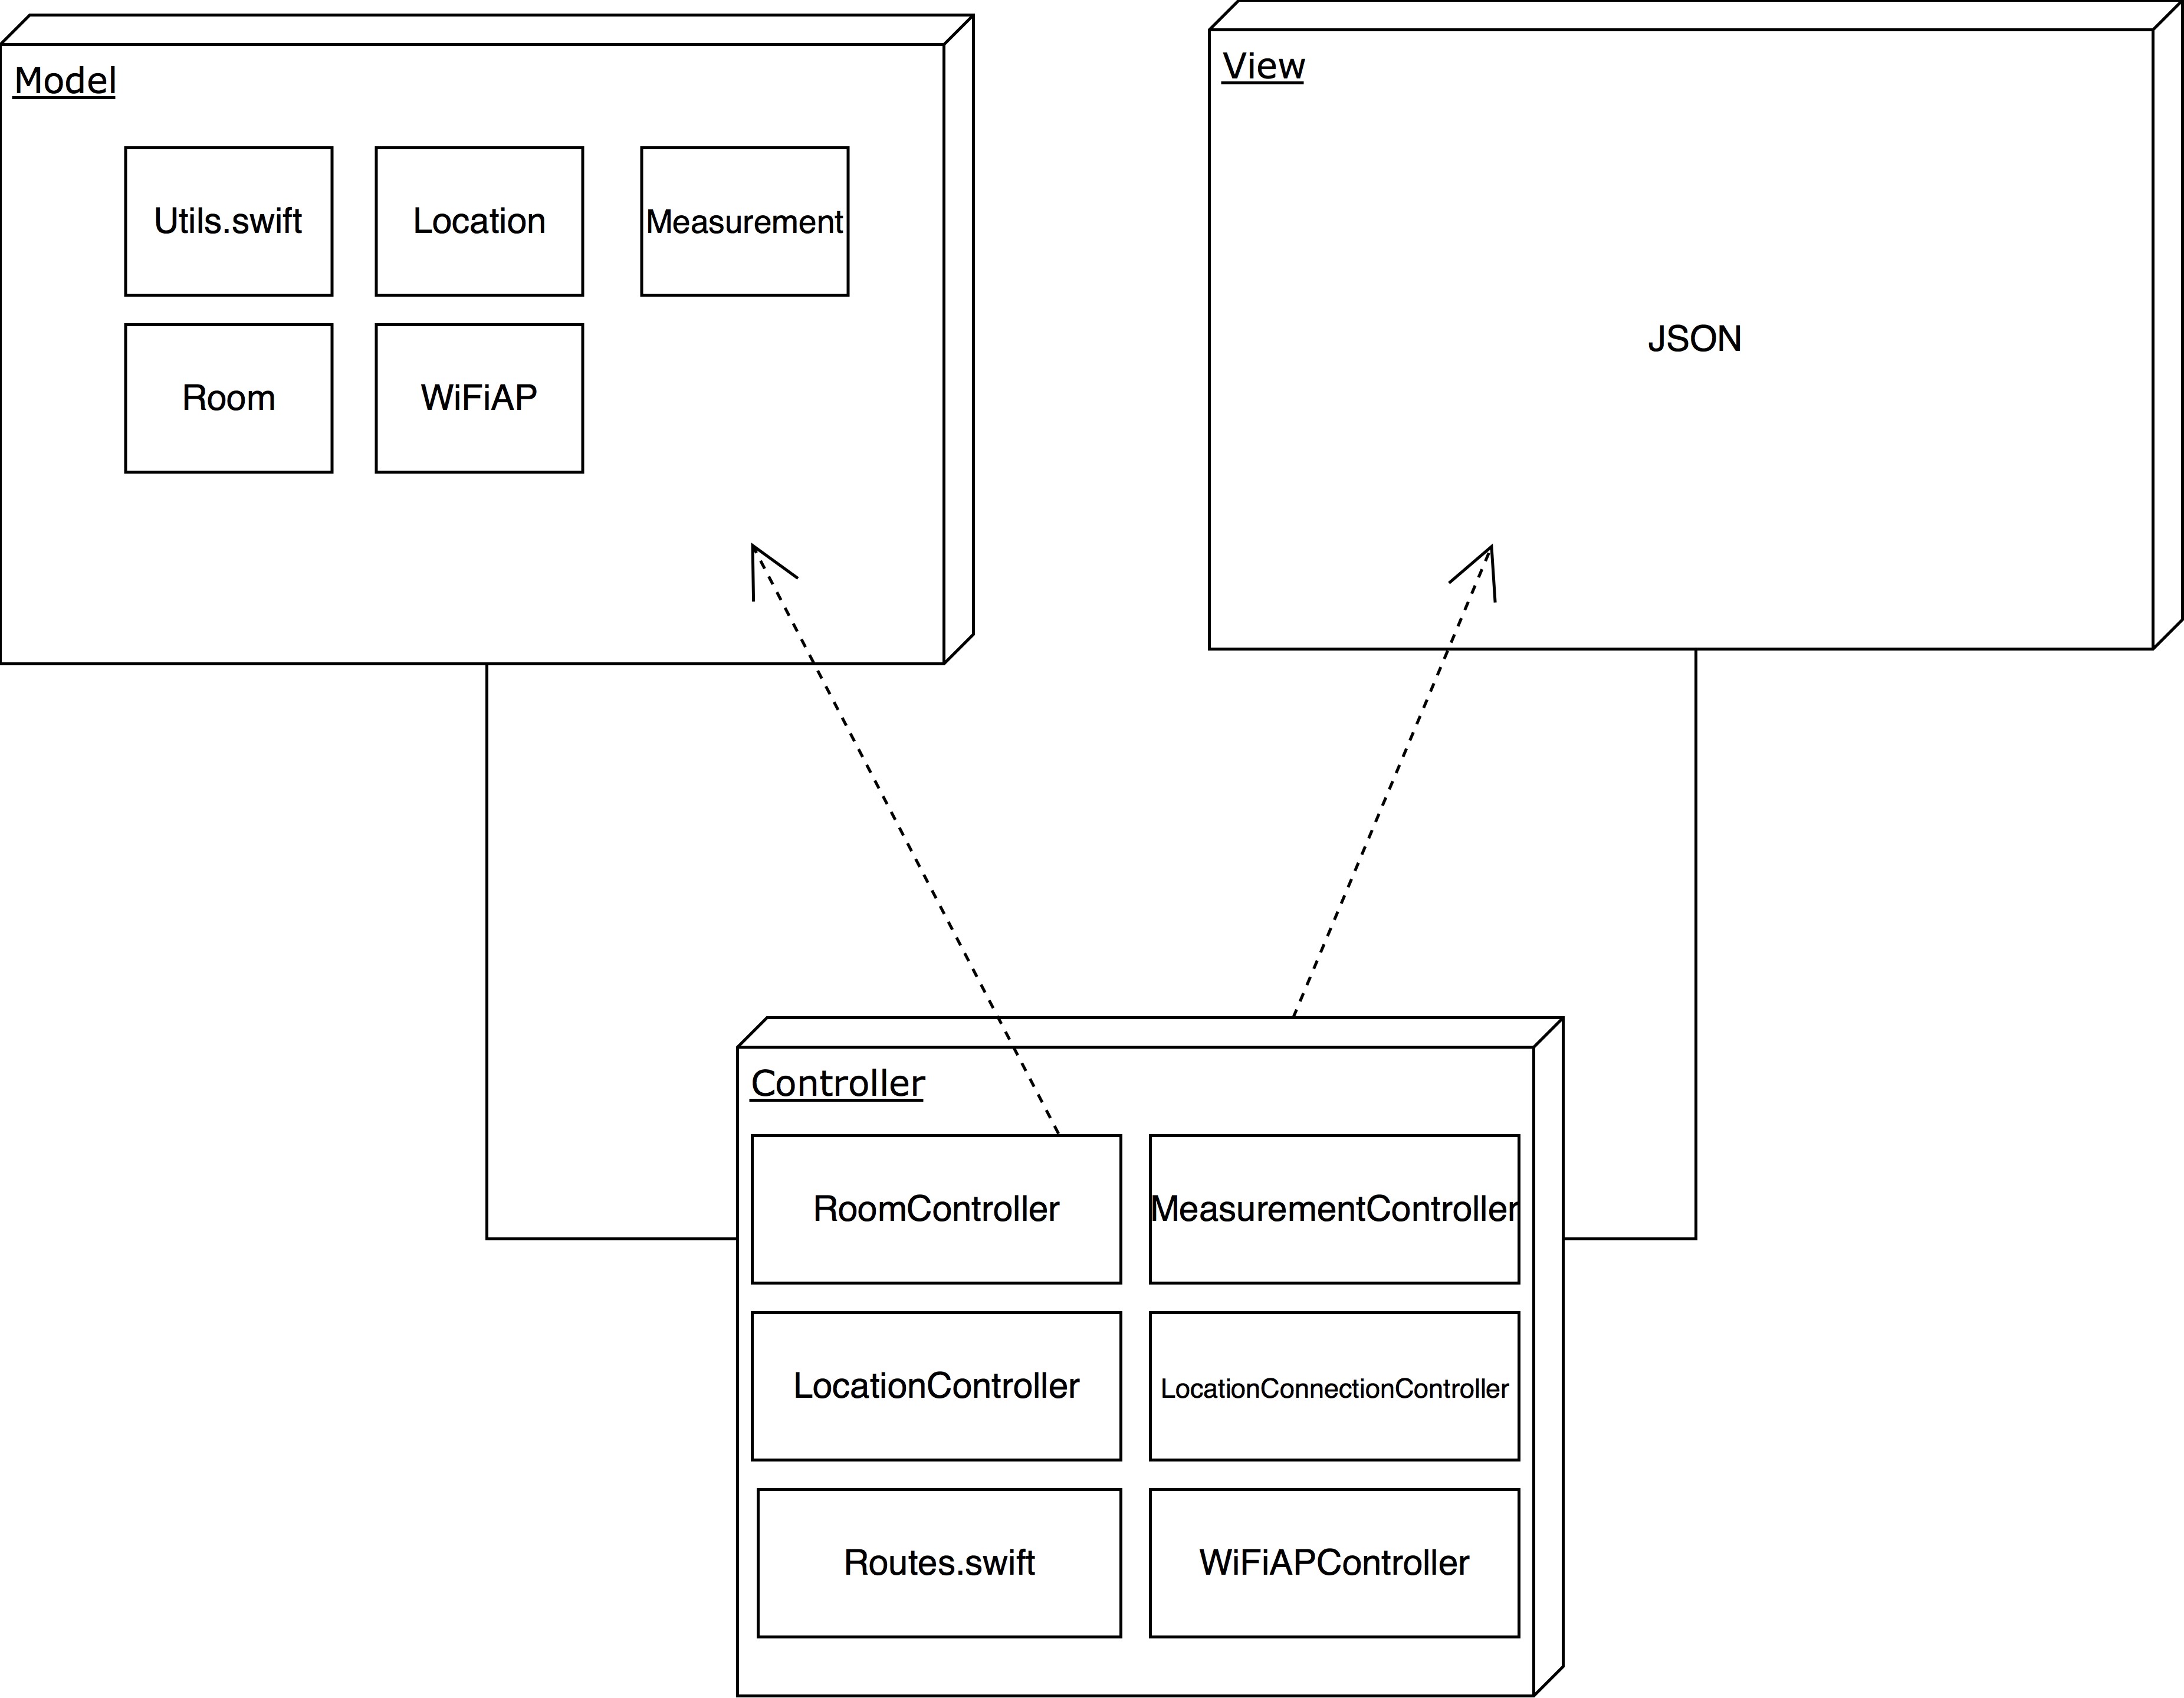
\includegraphics[width=420px, height=332px]{Design/Back-end-Storage-MVC.png}}
    \centering
    \caption{Back-end Data Management Server MVC Design. The design is split into model, view and controller. The rectangles inside each component represent the classes that are part of it.}
    \label{fig:back-end-storage-mvc}
\end{figure}

The API handles HTTP methods to "http://address/resource", where the resource is targeted. Additionally, "/resource/id" can be accessed, if available, in order to access a certain resource, identified by the id. The resources that can be accessed are the following:
\begin{itemize}
    \item For resource "/locations":
    \begin{itemize}
        \item GET: Returns a JSON representation of all locations in the database.
        \item POST: Accepts a JSON representation of the Location object and creates a new instance with the specified values.
    \end{itemize}
    
    \item For resource "/locations/[id]":
    \begin{itemize}
        \item GET: Returns a JSON representation of the location that has the specified id.
    \end{itemize}
    
    \item For resource "/locations/floor/[floorNumber]":
    \begin{itemize}
        \item GET: Returns a JSON of all the locations that are on the specified floor.
    \end{itemize}
    
    \item For resource "/rooms":
    \begin{itemize}
        \item GET: Returns a JSON of all the rooms created in the database
        \item POST: Accepts a JSON representation of the Room object and creates a new instance with the specified values.
    \end{itemize}
    
    \item For resource "/rooms/[id]":
    \begin{itemize}
        \item GET: Returns a JSON of the room that has the specified id.
        \item PATCH: Replaces the values from the room identified by the specified id with the new values submitted.
        \item DELETE: Deletes the room that has the specified id.
    \end{itemize}
    
    \item For resource "/rooms/clearData/[roomID]":
    \begin{itemize}
        \item GET: Clears the data that is associated with the room that has the specified roomID.
    \end{itemize}
    
    \item For resource "/rooms/search":
    \begin{itemize}
        \item POST: Accepts a JSON with a query to search for and will return all the rooms as JSON that match the query.
    \end{itemize}
    
    \item For resource "/rooms/connectingLocation/[id]":
    \begin{itemize}
        \item GET: Returns the location as JSON from the room with the specified id that is connected to an outside connection (i.e. another room).
    \end{itemize}
    
    \item For resource "/rooms/floor/[floorNumber]":
    \begin{itemize}
        \item GET: Returns all the rooms as JSON that are on the specified floor number.
    \end{itemize}
    
    \item For resource "/accessPoints":
    \begin{itemize}
        \item GET: Returns a JSON with all the access points that are in the database.
    \end{itemize}
    
    \item For resource "/accessPoints/[id]":
    \begin{itemize}
        \item GET: Returns a JSON with the access point that has the specified id.
    \end{itemize}
    
    \item For resource "/measurements":
    \begin{itemize}
        \item GET: Returns a JSON of all the measurements in the database.
    \end{itemize}
    
    \item For resource "/measurements/[id]":
    \begin{itemize}
        \item GET: Returns a JSON of the measurement identified by the specified id.
    \end{itemize}
    
    \item For resource "/measurements/address/[macAddress]":
    \begin{itemize}
        \item GET: Returns a JSON of the measurements from the access points that have the specified mac address.
    \end{itemize}
    
    \item For resource "/locationConnections":
    \begin{itemize}
        \item GET: Returns a JSON of all the connections between locations.
    \end{itemize}
    
    \item For resource "/locationConnections/id/[locationID]":
    \begin{itemize}
        \item GET: Returns a JSON of all the locations that are connected to the location identified by the specified location id.
    \end{itemize}
    
    \item For resource "/linkLocations":
    \begin{itemize}
        \item GET: Links all the locations in every room between themselves.
    \end{itemize}
\end{itemize}

\subsubsection{Data Storage Objects}
\label{sec:data-storage-objects}
The database stores data used for positioning and navigation. The data models defined to be used in the database, together with the relations between them are shown in figure \ref{fig:erd-diagram}.

\begin{figure}[H]
    \centering
    \fbox{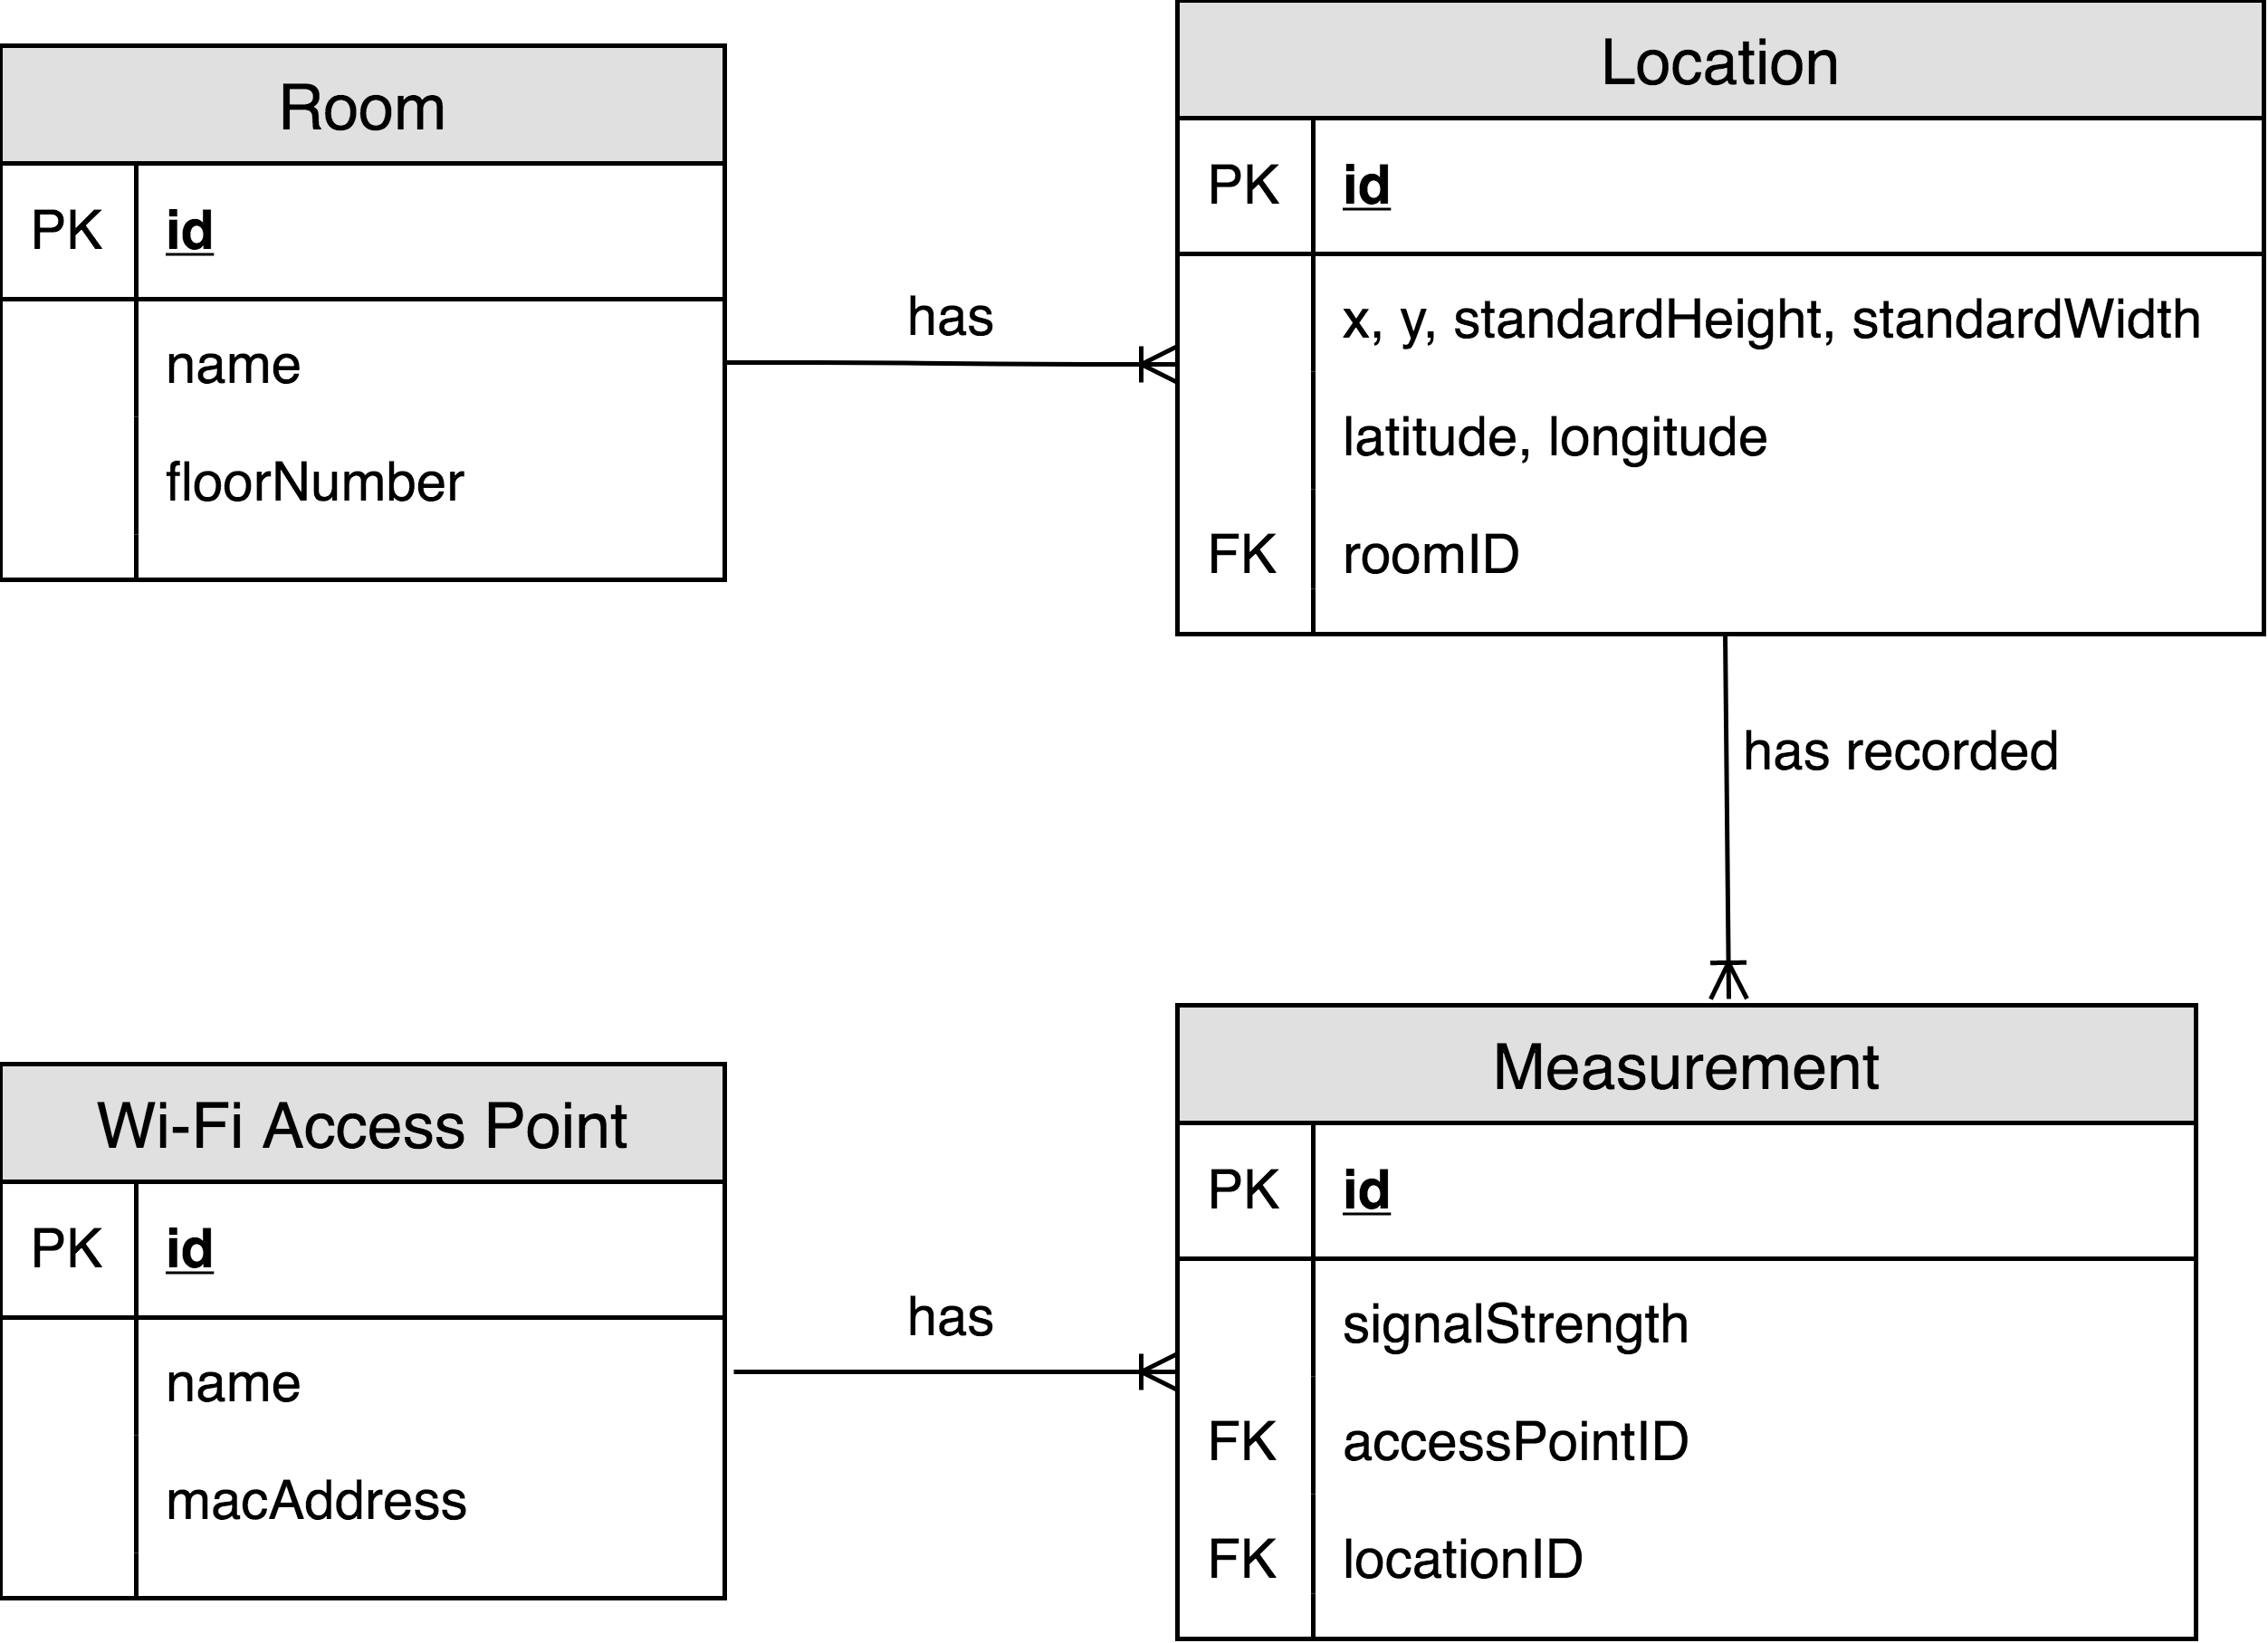
\includegraphics[width=350px, height=254px]{Design/ERD.png}}
    \centering
    \caption{ERD diagram of the database objects. The rectangles represent the data models along with their properties; they are connected between themselves by relations.}
    \label{fig:erd-diagram}
\end{figure}

For the data models just presented in figure \ref{fig:erd-diagram}, the following properties have been defined:
\noindent\textbf{Room:}
\begin{itemize}
    \item Name: the name of the room as a string.
    \item Floor number: the floor number where this room is located.
\end{itemize}

\noindent\textbf{Location:}
\begin{itemize}
    \item 2 coordinates (x, y) for the location measured on the image, along with 2 more values: width and height. These values represent the size of the screen the location has been recorded. Based on these values, x and y can be adapted to any screen size.
    \item Latitude
    \item Longitude
    \item Room ID: the link between a location and its corresponding room.
\end{itemize}

\noindent\textbf{Measurement:}
\begin{itemize}
    \item Signal strength: the value of the signal strength recorded.
    \item Access Point ID: the link between a measurement and its corresponding Wi-Fi access point.
    \item Location ID: the link between a measurement and the location where it was registered.
\end{itemize}

\noindent\textbf{Wi-Fi Access Point:}
\begin{itemize}
    \item Name: the name of the network as a string.
    \item MAC Address: the unique identifier of the network.
\end{itemize}

\newpage
\section{Data Flow}

\begin{figure}[H]
    \centering
    \fbox{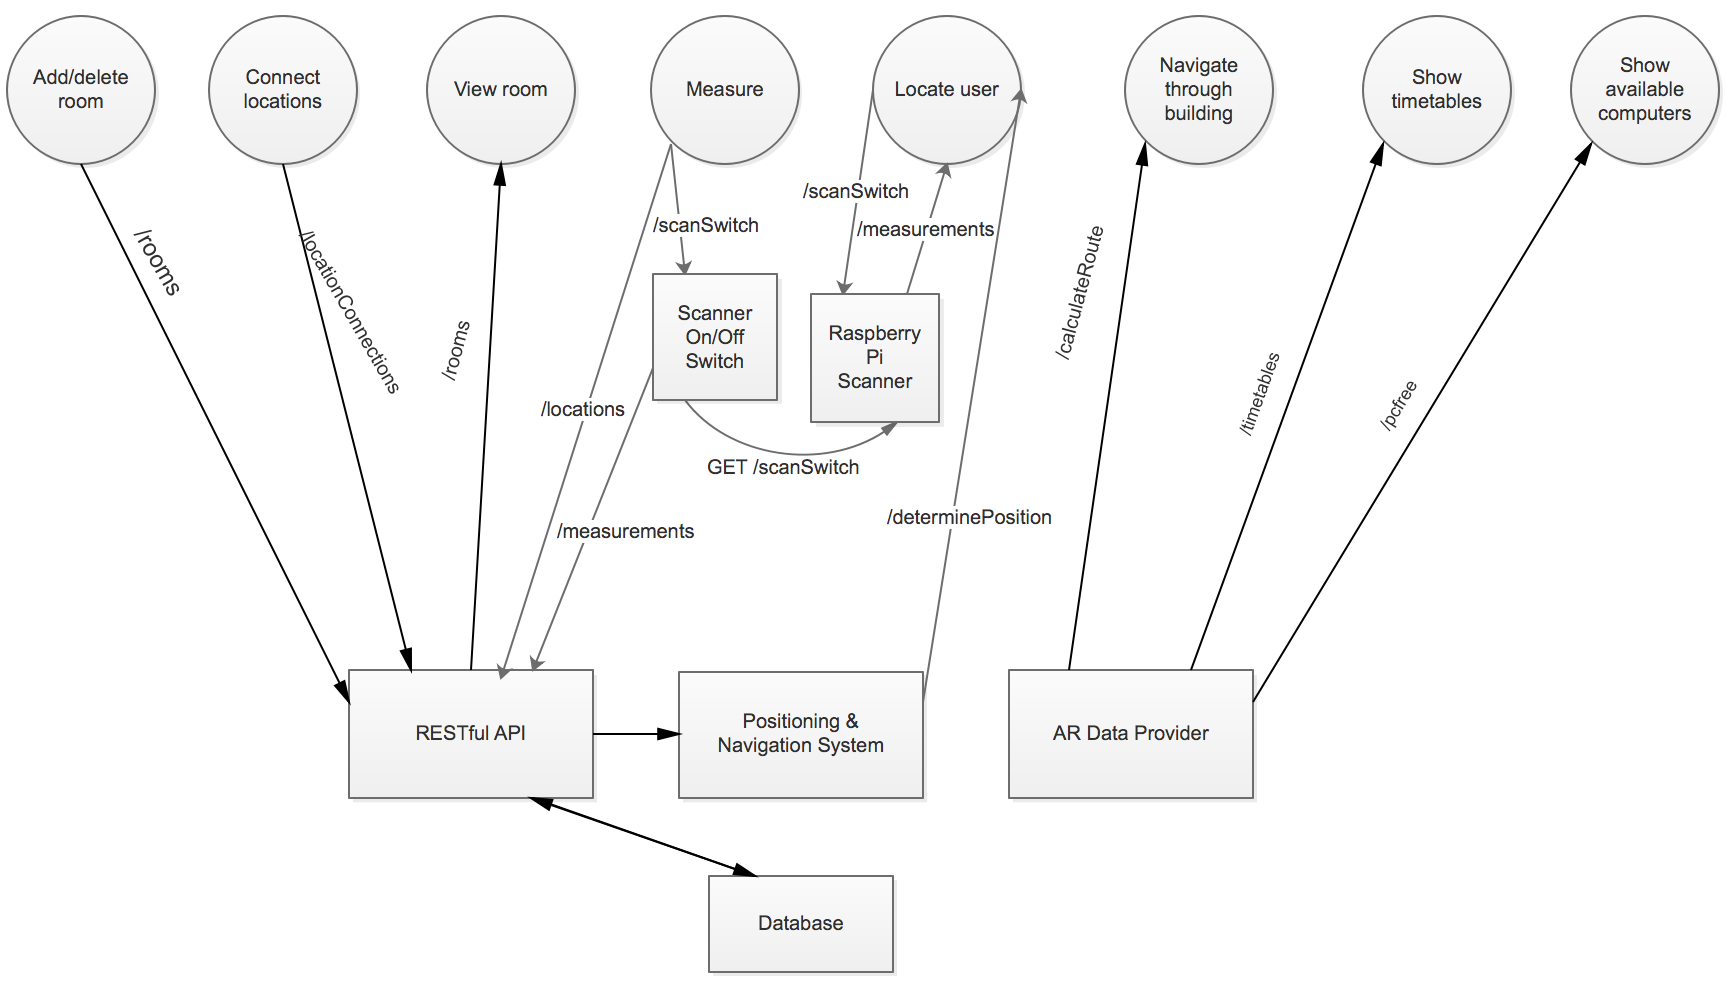
\includegraphics[width=420px, height=239px]{Design/data_flow_diagram.png}}
    \centering
    \caption{Data Flow Diagram. Represented in the figure is how the information is passing throughout the whole system. Circles represent the processes, and the rectangles and squares represent the data processing units.}
    \label{fig:data-flow-diagram}
\end{figure}

On the first run of the admin mobile application, the user will be greeted with a list of the available floors to measure. From there, on each floor rooms can be added by inputting their name. The data is then converted into JSON format and sent to the database through the RESTful API that receives a POST request to "/rooms", where data is parsed and saved into a Room object. After rooms are created, the admin application will request to fetch them by making a GET request to "/rooms" which will return a list of the registered rooms. This will facilitate registering for locations in the rooms the user will select.

Next, locations can be measured in the selected room by following the steps:
\begin{itemize}
    \item A Location object is created by making a POST HTTP request to "/locations".
    \item The Scan Switch is turned on by being set to true and the roomID and locationID that need to be assigned to the measurements scanned are sent. This is done by making a PATCH HTTP request on "/scannerSwitch/1".
    \item The Raspberry Pi detects that the Scanner is turned on, saves the roomID and locationID, and then the scanned data is assigned to those ids and the measurements are uploaded by using the RESTful API and making a POST HTTP request on "/measurements".
    \item Data is being processed from the JSON format and saved into the database.
\end{itemize}

After the locations are created and Wi-Fi measurements have been scanned, the next step is to connect certain locations in order to provide navigation. The admin user will then open the corresponding floor plan for the floor that they are on currently. This will send a GET HTTP request to "/locations/floor/[floorNumber]", where the desired floor number is specified. Given the set of locations, the admin user can select two of them that are on the floor plan in order to connect them. This will send a POST HTTP request to "/locationConnections" with the corresponding location ids that need to be connected together. 

The next steps are made by the user application, which will request to position the user after the application is launched. The positioning process starts by turning the Scanner Switch on, but this time by setting an additional flag, "storeData", to false. This will let the scanner know that the current measurement data will be only needed to compare it to the already existing data, and not stored in the database. After scanning is done, the measurement data is downloaded on the mobile phone as JSON, and then sent to the Positioning \& Path Finding System by making a GET HTTP request to "/determinePosition". The current position will be returned as JSON, parsed by the mobile application, and shown on the floor plan.

In order to facilitate navigation, a POST request will be made to the Positioning \& Path Finding System, which will contain a JSON of the current position and the finish position. The server will then return a JSON of the path to follow and the distance of the path. The application will show the route on the floor plan, along with the estimated time of arrival and the total distance. The navigation process in the user application can be put in "Augmented Reality" mode as well, where an arrow will guide the user. Whilst walking to the destination, visual information will be available, which are part of the AR features earlier mentioned. This data will be retrieved by making GET HTTP requests to "/timetable/[roomNumber]", which returns an image of the timetable for the specified "roomNumber", or to "/pcfree/[roomNumber]" which will return the number of available computers for the specified "roomNumber".

\section{Third Party Content}
The system uses some third party code components which allow it to meet part of the requirements and specifications. By using third party content, time is saved and productivity is increased. Below, the third party content used in this project are described.

\subsection{SwiftSpinner}
"SwiftSpinner" is an open source library to show visual cues as loading spinners when a background task needs to be executed. This allows to have a better user experience, because by using a spinner, the user knows that they have to wait for data to show in order to use a specific part of the application.

\subsection{ARKit + CoreLocation Library}
The system uses "ARKit + CoreLocation", which is an open source library that makes it easy to place elements of AR on locations, given the latitude and longitude. By default, the library using CoreLocation for positioning and handling locations. CoreLocation is a system framework implemented in iOS which uses the mobile phone's GPS and GLONASS chips for that, but this comes into conflict with what the project wants to achieve: an indoor navigation system that uses only IPSes. Therefore, the library has been modified in such a way that it will use the project's indoor location system, instead of CoreLocation. This modification will be explained in the Implementation chapter, where examples of the code will be provided as well.